\chapter{Installation of the AOM}\label{AOMInstallChapter}

We generate shifted beams by sending the seed light through an Acousto-optic Modulator (AOM)\footnote{also known as an Acousto-optic frequency shifter} using a double pass configuration. This is illustrated in Figure\,\ref{aomDiagramDetail}. A photograph of the AOM can be seen in Figure\,\ref{aom_upclose}.

\begin{figure}
\centerline{
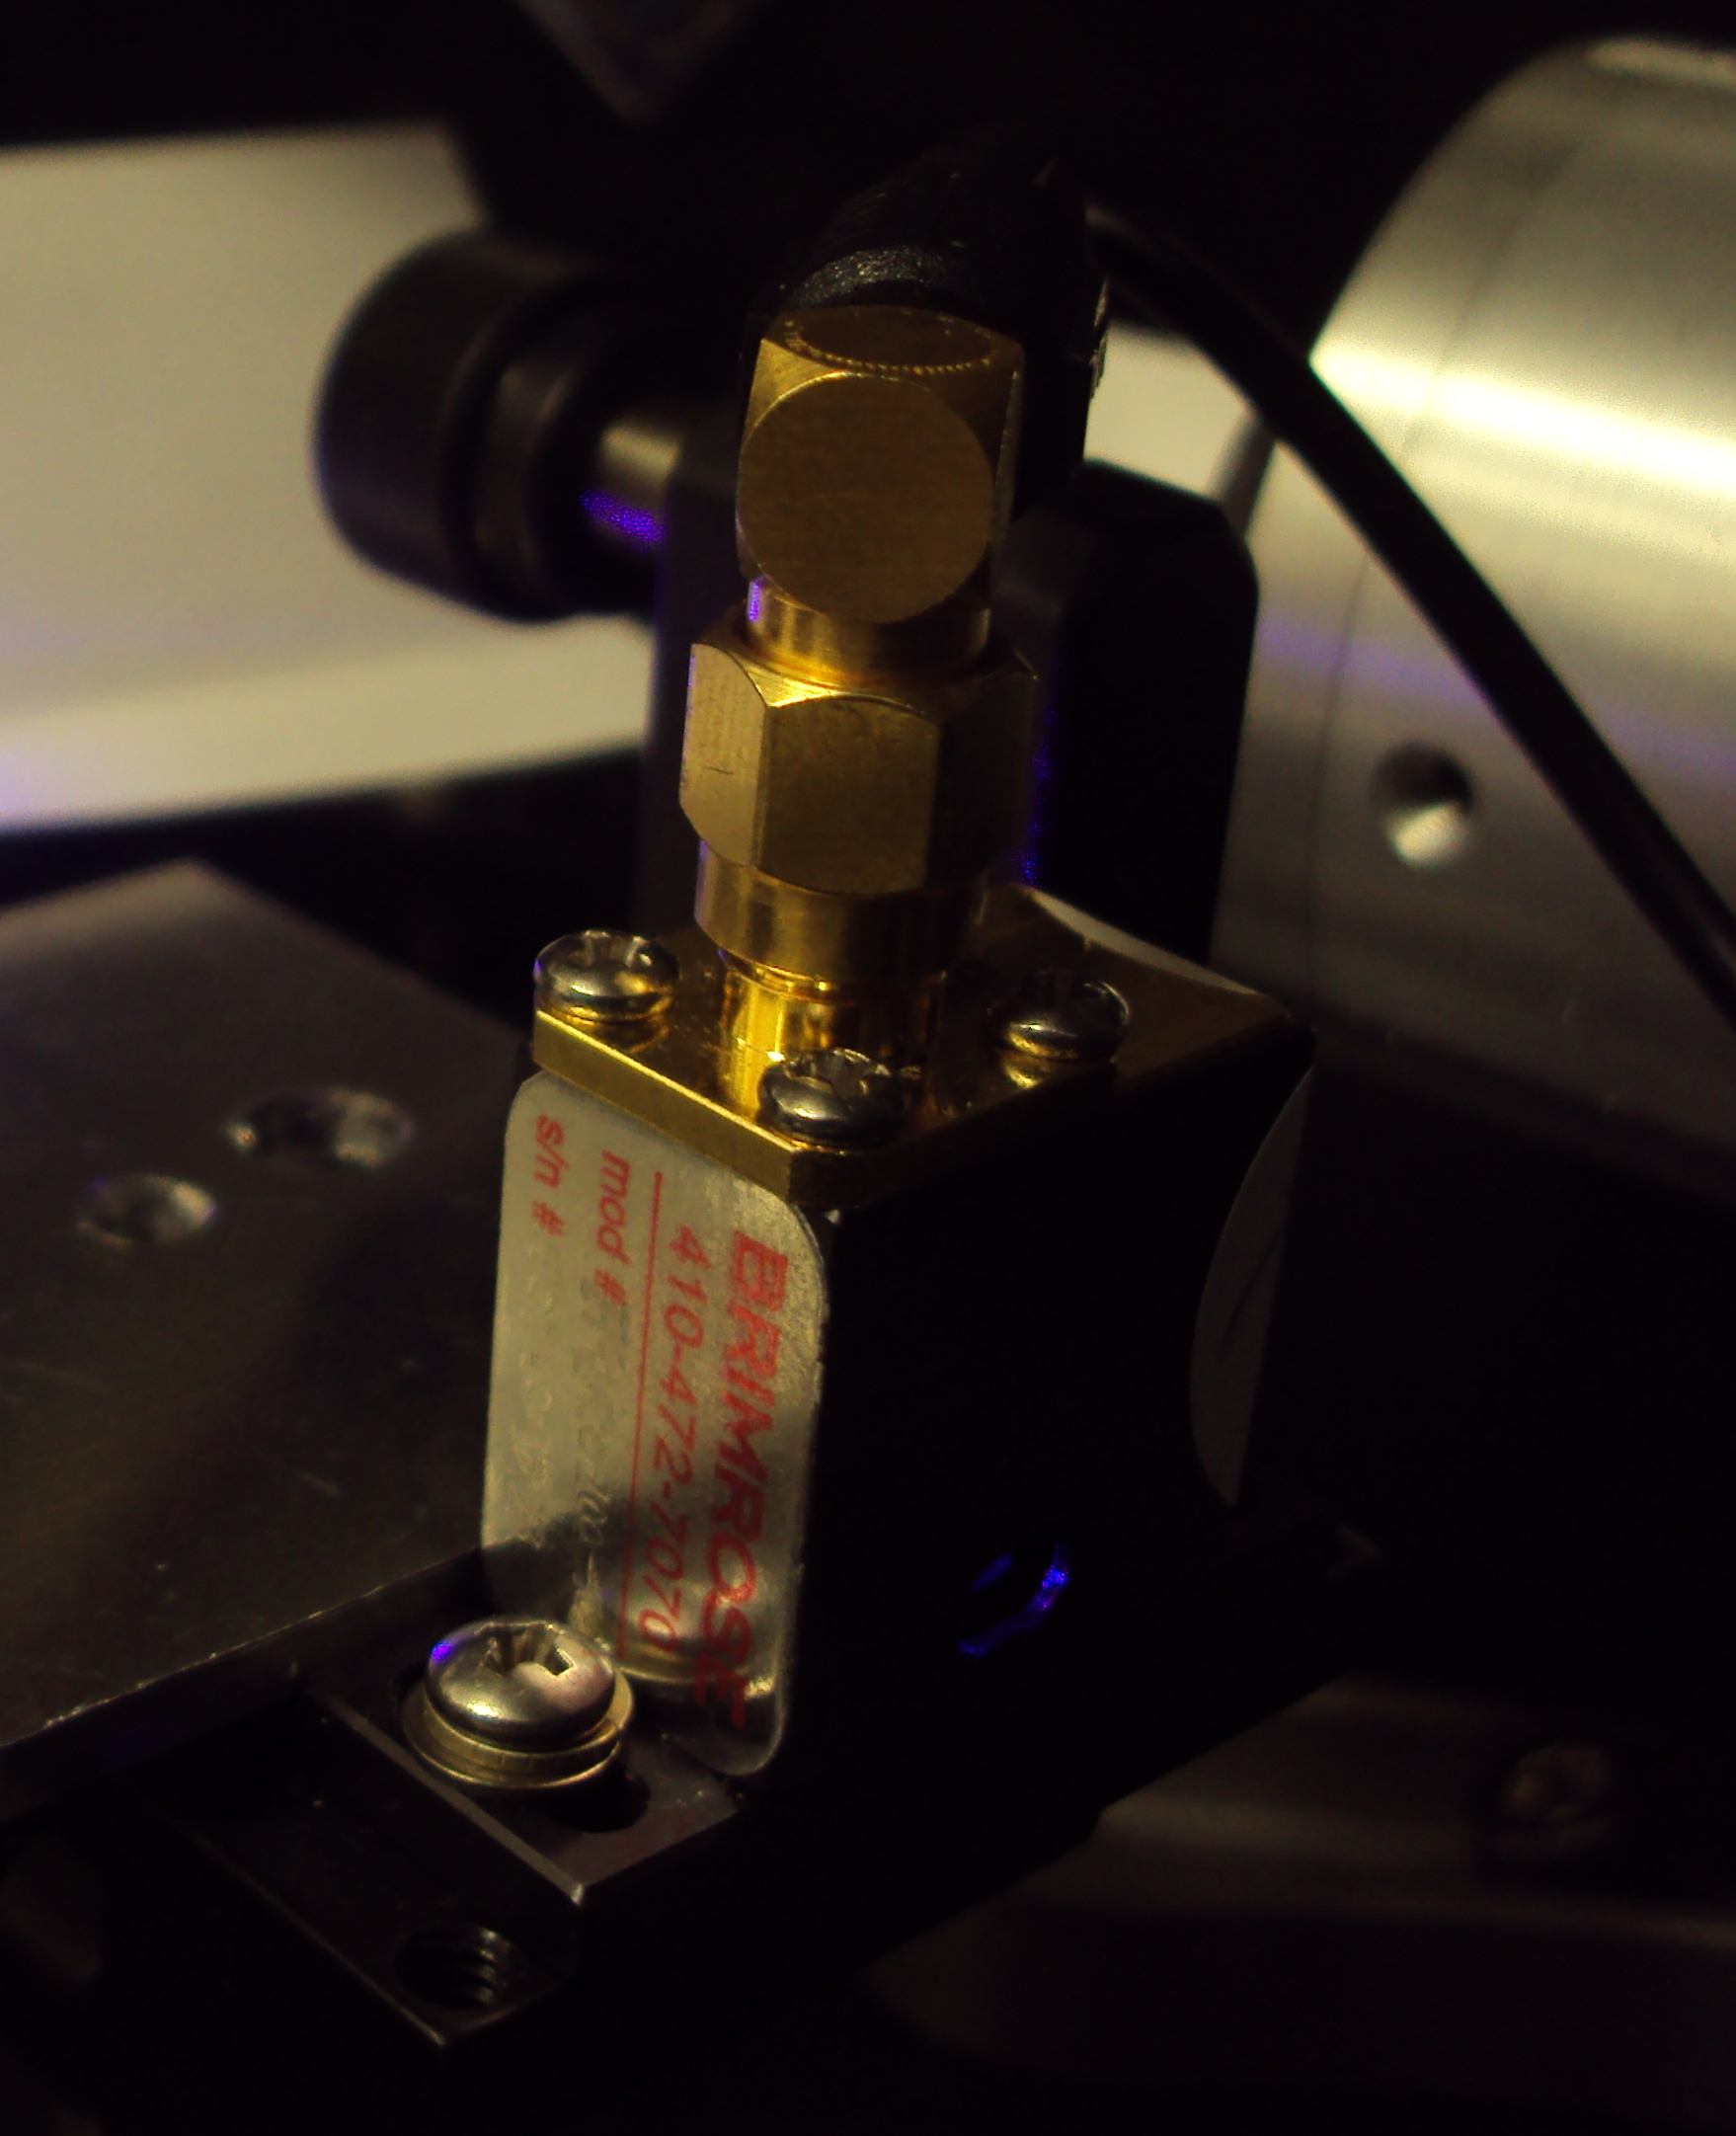
\includegraphics[width=0.95\textwidth]{aom_upclose.JPG}}
\caption[Photograph of AOM]{\label{aom_upclose} The AOM mounted in the setup. The aluminum plate in the lower left part of the photo that can be seen butting up against the AOM was used only as a guide for initial AOM alignment and was removed in the final system.}
\end{figure}
\begin{figure}
\centerline{
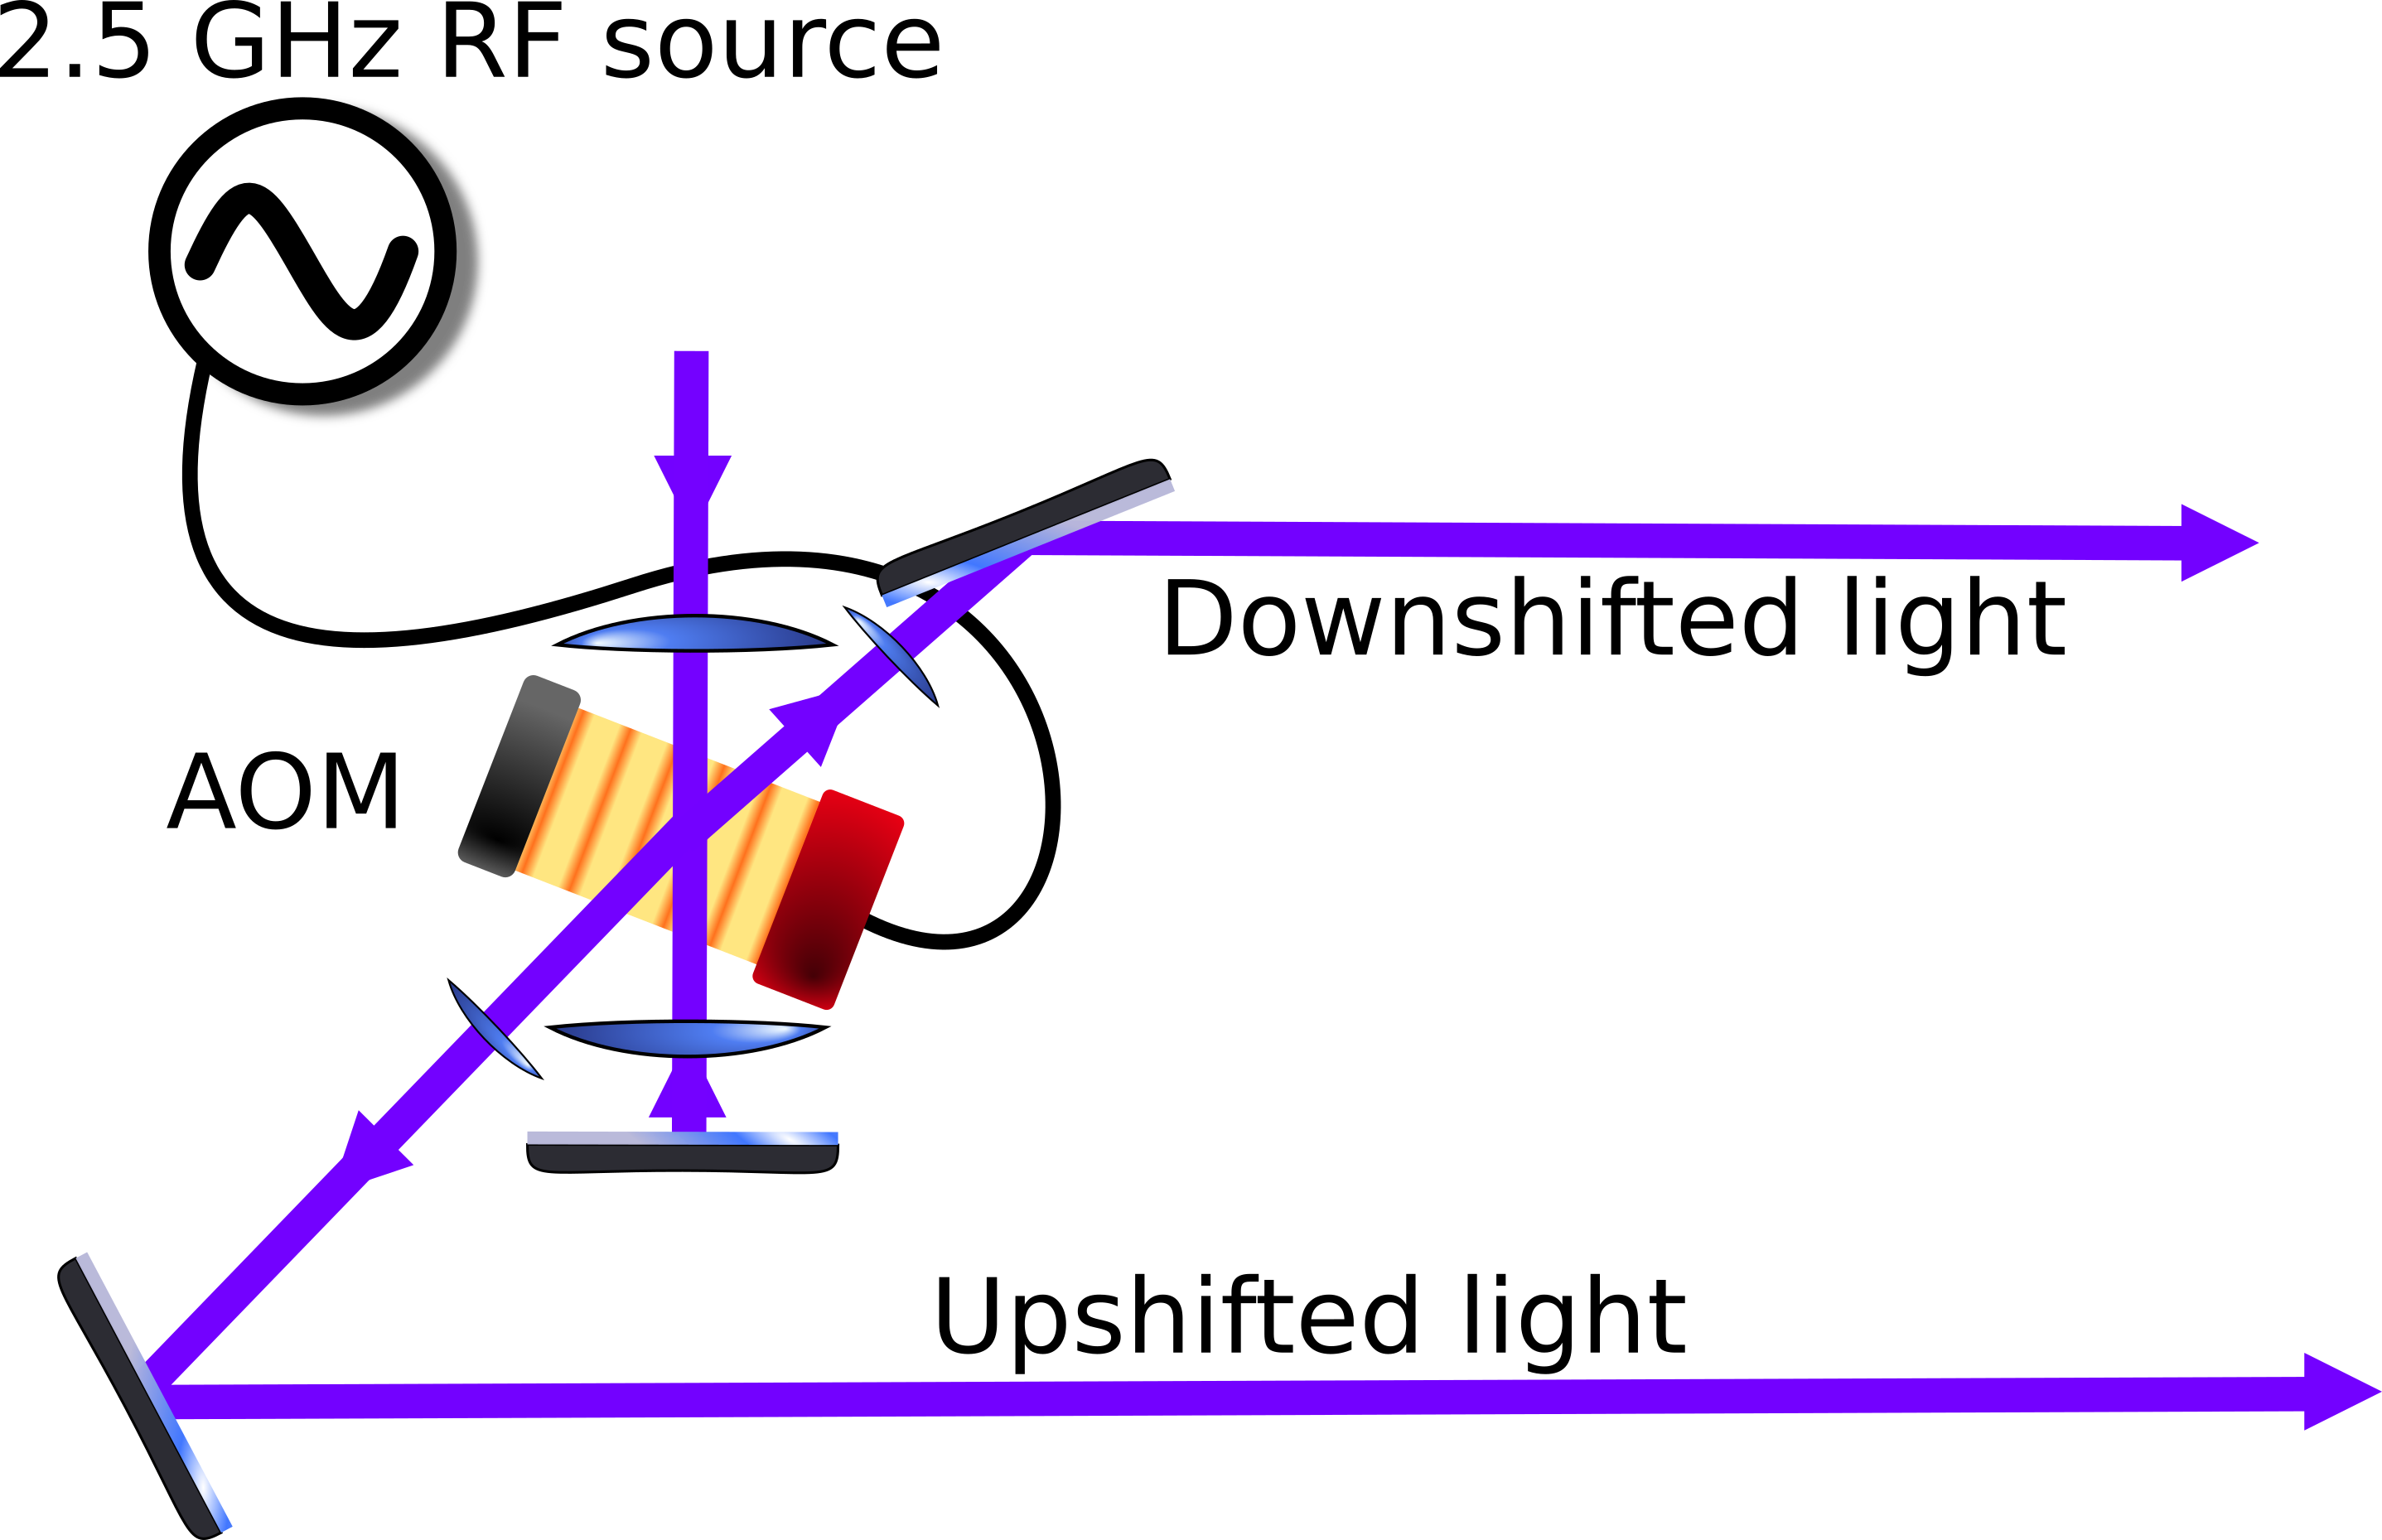
\includegraphics[width=0.95\textwidth]{diagramOfAOM}}
\caption[AOM diagram]{\label{aomDiagramDetail} Detail of Figure\,\ref{diagramOfSetup3}. The light from the master laser is depicted entering from the top of the diagram. This beam travels into the AOM, which is depicted in the center of the diagram. The up-shifted light (up-shifted in frequency, or blue shifted) is depicted travelling towards the lens and mirror near the lower left side of the diagram. The zeroth order diffracted beam is re-collimated and then retroreflected. The down-shifted light (red shifted) is depicted exiting the AOM towards the top right of the figure.}
\end{figure}

The AOM we use is model number TEF-2500-200-405 made by Brimrose Corporation of America. The crystal material is Tellurium Flouride; the center carrier frequency is 2500 MHz; the bandwidth (3dB) is 200 MHz. The AOM's anti-reflective coatings are specified to work at 405 nm. 
\section{Principle of operation}

The AOM is a crystal with a piezoelectric transducer attached to one side and an acoustic absorber attached to the other side. Acoustic waves are produced by the transducer. These waves travel across the active area of the AOM crystal and are absorbed by the absorber on the other side. The compression and decompression caused by the travelling acoustic waves changes the index of refraction within the crystal as a function of both space and time. This creates what are effectively a series of travelling Bragg planes that correspond to the acoustic wavefronts travelling across the crystal. Light crossing through the crystal can experience Bragg reflection off these planes and, because the effective reflective surface is moving, the light scattered off these features is Doppler-shifted. This light emerges at a distinct angle compared to the incoming light. This allows the AOM to produce frequency-shifted beams that are spatially separated from the unshifted components of the beam.

The relationship between the driving frequency and the Bragg angle for an AOM is well known and is given by 
\begin{equation}
m\lambda' = 2 \Lambda \sin \theta_B
%\sin{\theta}=\frac{m \lambda}{\Lambda}
\end{equation}
where $\theta_B$ is the Bragg angle (which is measured between the incoming beam and the Bragg planes), $\lambda'$ is the wavelength of the laser within the AOM crystal, $\Lambda$ is the wavelength of the acoustic wave in the crystal medium, and $m$ is an integer representing the diffraction order. The deflection angle (the angle between the unshifted portion of the beam and the outgoing shifted portion of the beam) is equal to twice the Bragg angle. Only $m=0,1$ are relevant to the experiment. The $m=1$ beams are the ones used to injection lock the slave lasers. The $m=0$ beam refers to the laser light that passes straight through the AOM with no frequency shift. Most of the power emerges in the $m=0$ diffraction order. The $m=0$ order beam from the first pass is retroreflected to produce the second pass.

The relationship between the driving frequency and the shift in the frequency of the light simply turns out to be 
\begin{equation}
    mf_{\textnormal{driving}}=\Delta f_{\textnormal{laser}}.
\end{equation}
%put in data sheet
Ultimately, getting the AOM to work properly involves optimizing just a few parameters. The AOM must be installed at the right angle relative to the incoming beam. I must ensure that as much of the incoming beam as possible hits the active aperture of the AOM, which is specified as having dimension 0.05 mm. This requires alignment in the X and Y directions, but it also means that I attempted to maneuver the AOM so that the focal point of the incoming beam was approximately in the center of the crystal in the Z direction as well (direction of propagation). This way, we keep the beam small on both of the entry holes in the case of the AOM. I also optimized the power used to drive the piezoelectric transducer. Furthermore, the intensity and shape of the incoming beam were adjusted to ensure that we do not exceed the maximum allowable intensity for the AOM, which is specified as 50 W/mm$^2$.
%shape instead of waist?
Thus, I will first discuss some work I did to characterize the incoming beam.

\section{Optimization of beam waist}\label{optimbeamWaist}
First, we would like to control the beam so that at its focus nearly all of the beam ($\sim99.96$\%) is within the active area of the AOM.
%\footnote{I did explore the possibility of just sending in a huge beam with lots of extra power in hopes that the part scattering off the active part of the AOM would work. Preliminary tests showed little promise for the technique. Furthermore, we would expect the possibility of severe distortion of the transverse mode of our laser.}
This area is specified as being 0.05 mm wide. Our goal is to have a beam waist radius that will be $\approx$4 times smaller than this 0.05 mm value.\footnote{Note that I am comparing the beam waist \emph{radius} to the full \emph{width} of the active area.} %diameter? 
If the beam waist is too small, we have to reduce the power to avoid damaging the AOM. Also, the diffraction efficiency decreases because the beam will interact with fewer Bragg planes. If the waist is too large, only a small portion of the beam would be within the active area of the AOM. This would reduce diffraction efficiency and cause distortion of the laser's transverse mode.

We can model the laser as a Gaussian beam. Gaussian beams have the property that their intensity profile always takes a Gaussian shape, i.e. \cite{lasersMilonniEberly}
\begin{equation}
\label{GaussianIntensity34}
    I(\mathbf{r})=I_0\exp\left(-\frac{2r^2}{w(z)^2}\right),
\end{equation}
where $z$ and $r$ are cylindrical polar coordinates. The variable $z$ represents position along the axis of propagation with the point $z=0$ defined to be the point along the beam path at which the beam is narrowest, while $r$ is the coordinate describing the distance from the $z$ axis. $I_0$ represents the intensity of the beam at $z=0, r=0$ and $w(z)$ is a function that gives the radius of the Gaussian beam, which is given by:
\begin{equation}
w(z)=w_0\sqrt{1+\frac{z^2}{z_R^2}}\label{beamwaist1D}.
\end{equation}
The beam radius, $w(z)$, is also the distance from the center of the beam to the point where the intensity of the beam has fallen by a factor of $1/e^2$ (i.e. the spot size). The Rayleigh range is denoted $z_R$, and also satisfies the relation 
\begin{equation}
z_R=\pi w_0^2/\lambda \label{rayleighRange1D}.
\end{equation}
A slight modification of Eq.\,\ref{GaussianIntensity34} allows us to model elliptical beams by allowing for a different waist in each of the $x$ and $y$ directions:
\begin{equation}\label{eqForI}
    I(\mathbf{x,y})=I_0\exp\left(-2\left(\frac{x^2}{w_x(z)^2}+\frac{y^2}{w_y(z)^2}\right)\right).
\end{equation}
Here, there are two relevant beam radii, $w_x$ in the $x$ direction and $w_y$ in the $y$ direction. Each of these has an associated Rayleigh range $z_{Rx}$ and $z_{Ry}$, and each satisfies relations analogous to Eqs.\,\ref{beamwaist1D},\ref{rayleighRange1D}.

I can measure the Gaussian beam radius in one dimension using a standard knife-edge technique. This involves placing a photo diode in the path of the beam. A razor blade is then moved perpendicular to the beam in a controlled way such that the beam is partially blocked. The blade is then moved across the laser beam in a direction perpendicular to the blade's edge to several different locations. For each razor blade position $x$ the power incident on the photo diode is measured. By integrating Eq.\,\ref{eqForI}, we get
%picture?

\begin{equation}
{\rm Power\ incident\ on\ photodiode}=\frac{1}{2} P \left(\erf \left( \frac{\sqrt{2} x}{W_{0x}}\right)\right).
\end{equation}
%get data for this?
We do this several times at various points along the path of the laser and can perform a curve fit to calculate our beam divergence and therefore infer its waist. 

I was somewhat worried that modeling the beam coming into the AOM as a Gaussian beam would not be adequate. This was in part due to irregularities in the transverse mode of the master laser.
%\footnote{The experiment still worked -- all that matters is that we are able to get the master laser stable and couple diffracted light from the AOM into the slave lasers. Ultimately, it was discovered by other students that this was due to a manufacturing defect in the optical isolators.}
Because I was planning to operate the AOM relatively close to its damage threshold, I examined the possibility of using a more sophisticated theory to model our beam based on measurable parameters. 

Siegman \cite{SiegmanBeamQuality} discusses the characterization of beams in terms of a quantity that is known simply as ``$M^2$.'' One way to interpret $M^2$ is that it serves as a measure of how Gaussian a beam is. If a beam is Gaussian, $M^2=1$. If a beam contains higher order Laguerre-Gaussian modes, $M^2$ will be greater than 1. In Ref.\,\cite{SiegmanBeamQuality}, Siegman asserts that any beam comprised of Laguerre-Gaussian modes can be mathematically proven to propagate according to the following equation:
\begin{equation}
W_x^2=W_{0x}^2+\left( \frac{M_x^2 \,\lambda}{\pi \, W_{0x}}\right)^2 (z-z_{0x})^2 \label{SiegmanBeamPropagate01}.
\end{equation}
The $z$ coordinate of the $x$-direction beam waist is given by $z_{0x}$. The spot size parameter (radius) of the beam in the $x$ direction is represented by $W_x(z)$, which can be written as  
\begin{equation}
W_x(z)=2 \sigma_x,
\end{equation}
where the second-moment width, $\sigma_x$, is defined by 
\begin{equation}\label{secondMomentWidth}
\sigma_x^2=\frac{\int_{-\infty}^{\infty} (x-x_0)^2 I(x,y)\, dx\, dy}{\int_{-\infty}^{\infty} I(x,y)\, dx \, dy}.
\end{equation} 
Here $I(x,y)$ is the intensity profile of our beam, which is propagating in the $z$ direction. 
The second moment width $\sigma_x^2$ then satisfies the following equation:  
%shoot----this factor of 4. I might be all wrong on my calculations. 
\begin{equation}
\sigma_x^2=\sigma_{0x}^2+\left( \frac{M_x^2 \,\lambda}{4 \pi \, \sigma_{0x}}\right)^2 (z-z_{0x})^2 \label{SiegmanBeamPropagate00}.
\end{equation}
In the special case of the Gaussian beam, $2\sigma_x(z)=w_x(z)$.

In principle, we could take measurements of $\sigma_x^2$ for our beam using the knife edge technique described above at several points along the beam's path and then fit this to Eq.\,\ref{SiegmanBeamPropagate00}.
I tried allowing $M^2$ to be one of my fit parameters as I analyzed data from the beam, but I found it difficult to get data of sufficient quality to give a good estimate. The knife edge data did not have sufficient resolution over a large enough range. One problem is that the contribution to $\sigma_x$ increases as the square of the distance from the center of the beam. This means that any measurement has to be very accurately adjusted to compensate for background offset. I also attempted to use a camera, but I was not able to trust its linearity and offsets enough to get good results. Information about my attempt to calibrate the camera can be found in Appendix\,\ref{BeamWaistAppendix}. 

However, I did consider the implications on the beam if $M^2\neq 1$. I can look at the effective slope of divergence by rearranging Eq.\ \ref{SiegmanBeamPropagate00} and taking the limit as $(z-z_R) \rightarrow \infty$
\begin{equation}
\frac{\sigma_x}{z-z_R}=M_x^2 \frac{\lambda }{4 \pi \sigma_{0x}} \label{SiegmanBeamSlope}.
\end{equation}
%note: check this again. 
%does z0 matter as a fit parameter? I don't think so. 
Note that the smallest possible beam waist radius corresponding to any given beam divergence occurs if $M^2=1$. That is, if I measure the beam divergence and perform my curve fit assuming that $M^2=1$, the beam-waist radius that I calculate will be guaranteed to be \emph{smaller than or equal to} the actual beam waist radius of the beam no matter what the beam's actual value of $M^2$ might be. Thus, for the purposes of keeping the intensity at the beam waist below the AOM's damage threshold, the assumption that $M^2=1$ gives a sort of ``worst case scenario.'' 

\subsection{Ray transfer matrix analysis of system}
It is crucially important that I limit the intensity of the light that passes through the AOM. As a sanity check, I now calculate what the beam waist should be for our optical setup using an ABCD matrix (ray-transfer matrix). This model can be used to estimate the sensitivity of the system to small changes in the setup. In this way, I can verify that the system is robust against small changes and realignments and thereby gain some small reassurance. For example, if the master laser ever had to be taken apart and reassembled, it would likely be the case that there will be tiny differences in the position of the laser or collimating lens. I seek to verify that such small changes will not yield catastrophic changes in the size of the beam as it passes through the AOM.  

%This is in a lab notebook somewhere. You need to find it there, I think. Or it's in a Mathematica file. 
%found: the Mathematica files are generalABCDfinding.nb, ABCDwillWeBreakAOM.nb . The m files, well, I think the ones I want are in checkTheWaists_realDATA. 

There is a method of modeling Gaussian beam propagation using a matrix
\begin{equation}
M=\begin{bmatrix}A&B \\C&D\end{bmatrix}
\end{equation}
which is known as a ``ray transfer matrix'' or simply as an ``ABCD matrix.'' We will use the well-known rule \cite{BYUOpticsBook,lasersMilonniEberly} for modelling a Gaussian beam as it passes through a system described by a ray transfer matrix with elements $A$,$B$,$C$ and $D$, which is 
\begin{equation} \label{ABCDlawforGaussianBeams}
z_0'-iz_R'=\frac{A(z_0-iz_R)+B}{C(z_0-iz_R)+D}.
\end{equation}
Here, $z_0'$ represents the location of the beam waist relative to the end of the system described by the ABCD matrix and $z_R'$ represents the new Rayleigh range of the beam. The location of the beam waist relative to the start of the system described by the ABCD matrix and the Rayleigh range of the incoming beam are represented by $z_0$ and $z_R$ respectively.
This can be solved to give 
\begin{align}
z_R' &= \frac{ z_R (BC-AD)}{C^2z_0^2+C^2z_R^2+2 C D z_0 + D^2} \\
z_0' &=\frac{AC z_0^2+ACz_R^2+ADz_0+BCz_0+BD}{C^2z_0^2+C^2z_R^2+2 C D z_0 + D^2}.
\end{align}
(Note that in an ABCD matrix, $A$ and $D$ are unit-less, while $B$ has units of $[\textnormal{length}]$, and $C$ has units of $[\textnormal{length}]^{-1}$.)

%This calculation should give us a feel for how sensitive we are to drifts in the optical setup. We will also be able to verify that the beam waist near the AOM is close to what we would expect based on the beam waist at the laser diode.

The system has only a few components that we need to model. At the start, we assume that the light coming out of the face of the laser diode is essentially a Gaussian beam with different beam waist radii for the $x$ and $y$ directions. The waist of this beam can be estimated based on parameters given in the data sheet. The data sheet for the master laser shows that a typical angle of divergence for light coming out of the laser is going to be 9$^\circ$ in one direction and 19$^\circ$ in the other. A Gaussian beam's angular divergence can be surmised by looking at Eq.\ \ref{SiegmanBeamSlope}. The relationship turns out to be the one given in Ref.\,\cite{MellesGriotGaussian}:
\begin{align}
\theta_{x} &= \frac{\lambda}{\pi w_{0x}}\\
\theta_{y} &= \frac{\lambda}{\pi w_{0y}}.
\end{align}  
Using this equation, we calculate the equivalent Gaussian beam height and width at the face of the laser based on the given angle of divergence of light. The beam waist dimensions turn out to be 972.913 nm and 460.854 nm at the face of the laser.

The light from the laser head is emitted and collimated by a lens\footnote{Thorlabs C570TM-A} with focal length 2.84 mm.  %before, I had 2.87 mm, IDK why
The propagation of the light from the laser diode to the collimating lens can be represented by the matrix
\begin{equation}
\begin{bmatrix}\label{ABCD1}
1 & d_1 \\ 0 & 1
\end{bmatrix},
\end{equation}
where $d_1$ represents the distance between the face of the laser and the collimating lens. The effect of the collimating lens is represented by the following ABCD matrix:
\begin{equation}
\begin{bmatrix}\label{ABCD2}
1 & 0 \\ -1/f_{a} & 1
\end{bmatrix}.
\end{equation}
Here, $f_a\approx$ 2.84 mm is the focal length of the lens

The beam then goes through various optical components, including the diffraction grating, the optical isolators, some wave plates, a polarizing beam cube, and many mirrors. The collective impact of these components on the waist of the beam can be modeled as simple propagation over some effective distance. %Even though propagating through a medium like the crystals in the optical isolators is different than propagating through air, travelling some distance through any medium is represented by the same ray transfer matrix as travelling some effective distance through air. 
In order to be complete, I will evaluate the outgoing beam properties over the entire range of possible path lengths. This is much easier than trying measure the total path length accurately and then trying to find detailed dimensions and indices of refraction for all the components in the system. The ABCD matrix representing this propagation is given by
\begin{equation}
\begin{bmatrix}\label{ABCD3}
1 & d_2-d_1 \\ 0 & 1
\end{bmatrix},
\end{equation}
where $d_2$ represents the total distance the beam travels from the face of the laser diode up until it reaches the lens that focuses it into the AOM. Thus, $d_2-d_1$ represents the distance from the collimating lens of the master laser to the lens that focuses the beam into the AOM. 
I estimate that the effective distance of propagation should be on the order of 1 m. To be safe, I will ultimately examine what happens for all beam paths between 0.5 m and 2 m. 

Finally, the beam is focused by a lens with focal length 10 cm and passed through the AOM. The focusing of the 10cm focal length lens is represented by
\begin{equation}
\begin{bmatrix}\label{ABCD4}
1 & 0 \\ -1/f_{f} & 1
\end{bmatrix},
\end{equation} 
where the focal length of the lens is written as $f_{f}$.

We can write the ABCD matrix for the whole system as the product of the ABCD matrices that represent the individual components of the system that were found in Eqs.\,\ref{ABCD1},\ref{ABCD2},\ref{ABCD3}, and \ref{ABCD4}: 
\begin{equation}\label{ABCDMatrixSystem}
\begin{bmatrix}
1 & 0 \\ -1/f_{f} & 1
\end{bmatrix}
\begin{bmatrix}
1 & d_2-d_1 \\ 0 & 1
\end{bmatrix}
\begin{bmatrix}
1 & 0 \\ -1/f_{a} & 1
\end{bmatrix}
\begin{bmatrix}
1 & d_1 \\ 0 & 1
\end{bmatrix}
=
\begin{bmatrix}
A & B \\ C & D
\end{bmatrix}.
\end{equation}

Finding the resulting ray transfer matrix that describes the system involves simply performing the matrix multiplication prescribed in Eq.\,\ref{ABCDMatrixSystem}. However, I opt not to write out result in this thesis. Instead, I used Mathematica to find the expressions for $z_R'$ and $z'$. These expressions were then evaluated numerically for several values of likely experimental parameters. In particular, I was interested in verifying that the beam waist inside the AOM remains reasonable for realistic values of $d_1$ (the distance from the laser face to the collimating lens) and $d_2$ (the distance traveled between the collimating lens and the other lens), since these are values that may not be known to high precision and which may drift with time. %may change as the system is maintained or repaired.

From this analysis, I calculated the effective area of the beam for many values of $d_1$ and $d_2$. For each of these values, I calculated the corresponding ratio between the intensity at the most intense part of the beam and the total power in the beam. The way to interpret this is that if we have a constant amount of power, the ratio shows how much the maximum intensity of the beam changes for different beam parameters. The data in Fig.\,\ref{waists111} shows that the maximum intensity of the beam changes smoothly as a function of $d_2$ and that for small drifts in $d_2$, the changes in the beam's maximum intensity are reasonable. 
%what about the position of the minimum? 
%If the calculations are correct, %what am I? A cartoon? 
Figure\,\ref{waists2} shows a plot of the effective area of the beam as a function of $d_1$ (the distance from laser face to collimating lens). The effective area is given by the expression $\pi W_{0x}W_{0y}/2$. The intensity at the center of the beam waist, $I_{max}$ is given by $I_{max}=\textnormal{power}/\textnormal{effective area}$. Figure\,\ref{waists2} shows that the effective area of the beam is sharply peaked when $d_1=f_a$, which means that the intensity is at a local minimum. If we assume that the laser was reasonably well-collimated when we did the initial optimization, we can deduce that the intensity of the laser at its focus will increase if the distance $d_1$ were to drift in the actual setup. Thus, any adjustment to $d_1$ should be accompanied by a reassessment of the power and waist of the beam hitting the AOM. The extent to which the beam is collimated can be evaluated visually by shining the beam on a wall that is about $\sim$1 m away. The collimating lens on the laser is mounted on a mount that fits into a 40 turns/inch threaded hole. Adjustments to the collimation are made by turning the lens holder.  Based on my experience collimating the laser, I am relatively confident that I can get the lens holder to within 1/10 of a turn of where it needs to be to collimate the laser perfectly.  An accuracy of 1/10 turn corresponds to getting the distance $d_1$ to within 0.010 mm of the focal length of the collimating lens. Clearly, this places $d_1$ somewhere within the main spike on the plot in Figure\,\ref{waists2}, but it does not lend enough confidence in the repeatability of this adjustment to allow an experimenter to forego reassessing the beam parameters at the AOM. 

\begin{figure}
    %\centerline{\includegraphics[trim=100pt 100pt 100pt 100pt, clip=true, totalheight=0.5\textheight,angle=90]{testfigure}}
    %\centerline{\includegraphics[totalheight=0.3\textheight]{testfigure}}
    \centerline{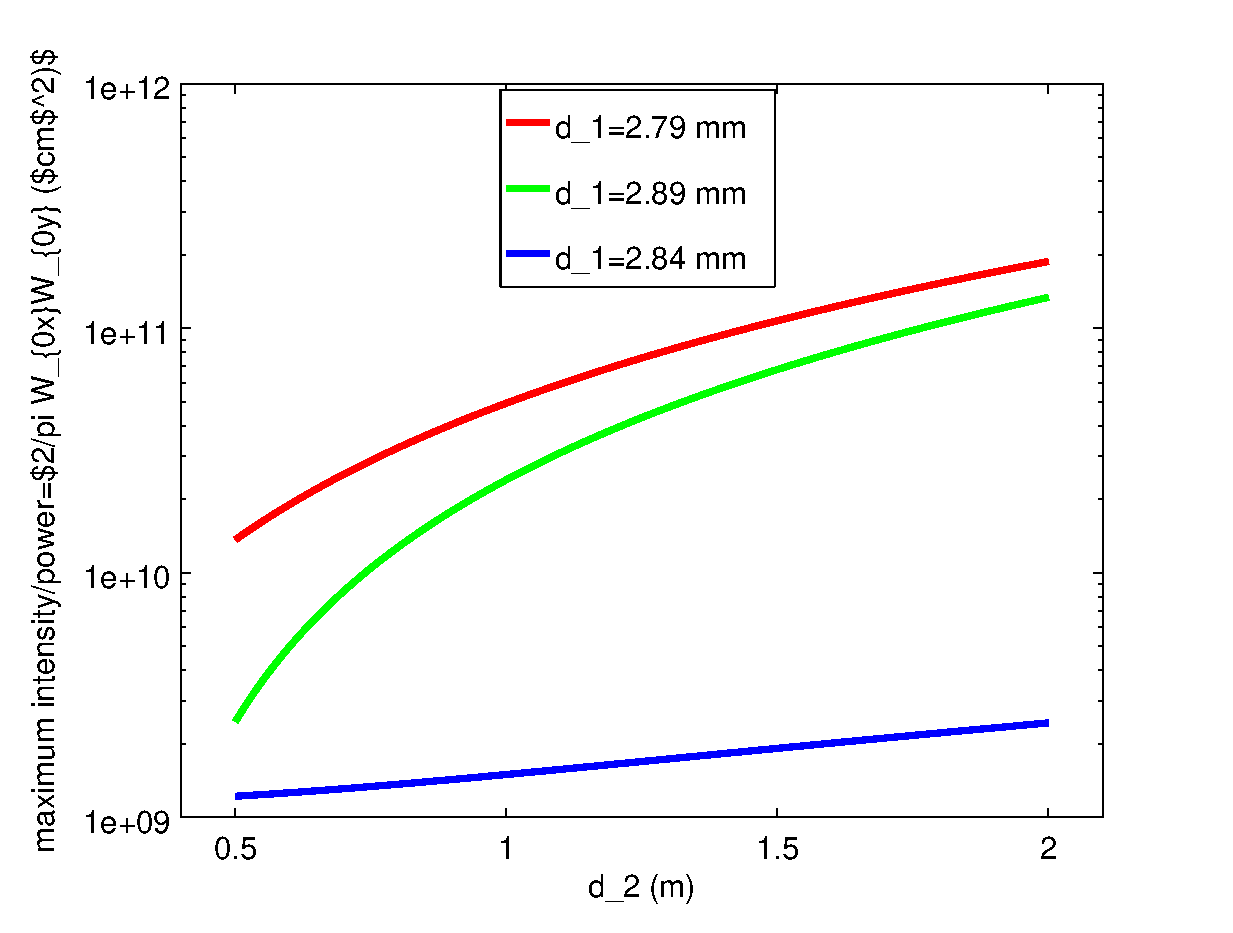
\includegraphics[width=0.95\textwidth]{waists1.eps}}
    %\includegraphics[totalheight=0.3\textheight]{testfigure}
    \caption[Maximum intensity$/$total beam power vs distance]{\label{waists111} The ratio of the maximum intensity to the total beam power as a function of the distance between the laser's collimating lens and the focusing lens ($d_2$) plotted for several values of $d_1$, which is the distance between the laser diode's output face and the collimating lens. The maximum intensity divided by the total beam power is given by $2/(\pi W_{0x}W_{0y})$. Because it is difficult to measure $d_2$ accurately, we have plotted it over a very large range of possible values. However, the actual path length is likely to stay the same to within a few millimeters, over which scales the system is relatively insensitive to changes in $d_2$.} 
\end{figure}
%%%%%TODO FIX CAPTION D2 IS IN m NOT mm

\begin{figure}
    %\centerline{\includegraphics[trim=100pt 100pt 100pt 100pt, clip=true, totalheight=0.5\textheight,angle=90]{testfigure}}
    %\centerline{\includegraphics[totalheight=0.3\textheight]{testfigure}}
    \centerline{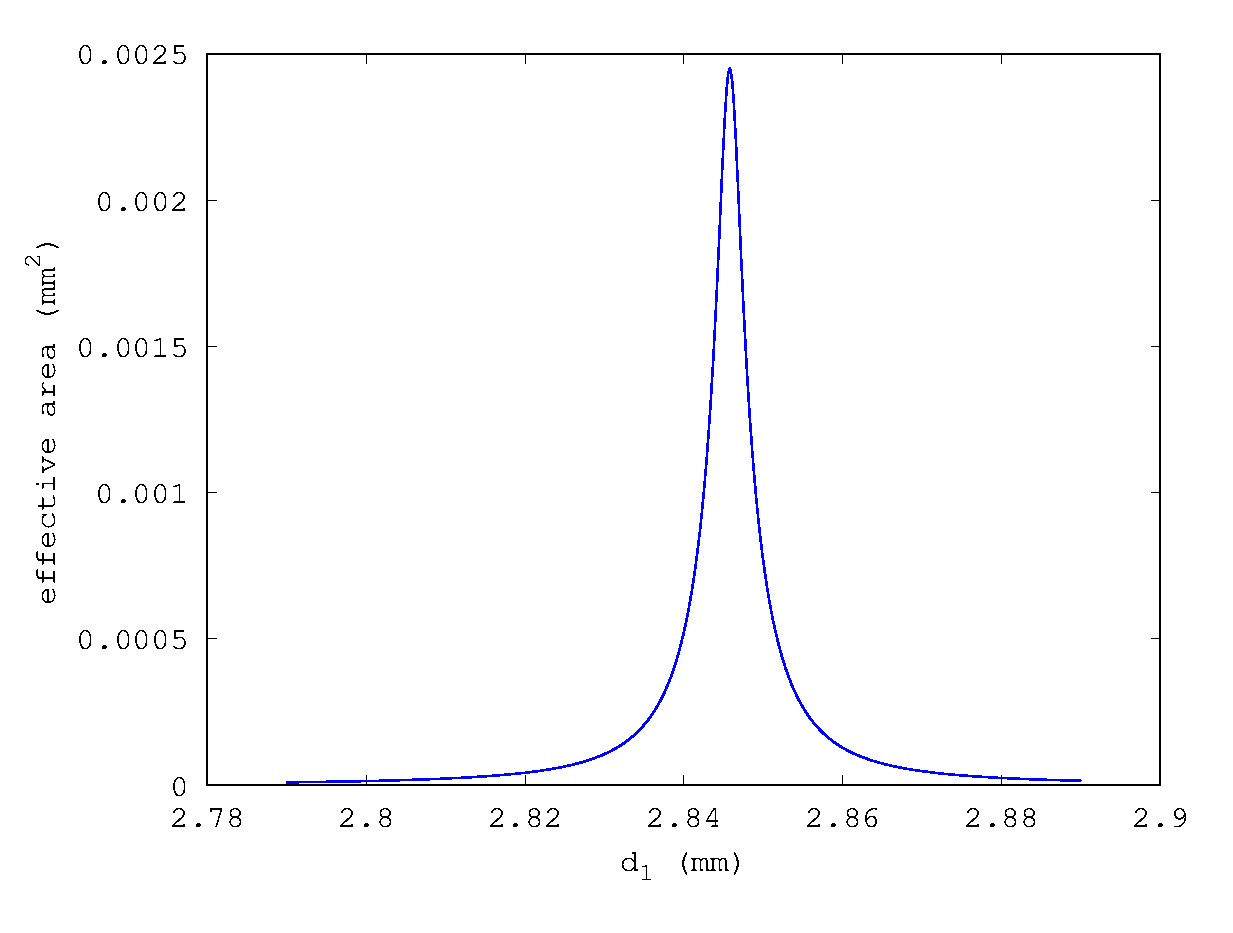
\includegraphics[width=0.95\textwidth]{waists2.eps}}
    %\includegraphics[totalheight=0.3\textheight]{testfigure}
    \caption[Effective beam area vs distance]{\label{waists2}
        The effective beam area at the beam's focus as a function of the distance between the laser diode's output face and the collimating lens ($d_1$).  Here, it is clear that the effective area is largest when $d_1$ equals the focal length of the laser's collimating lens. The peak intensity gets larger with any change of $d_1$.}
\end{figure}
